\documentclass[10pt, letterpaper]{article}

% Packages:
\usepackage[
  ignoreheadfoot, % set margins without considering header and footer
  top=1 cm, % seperation between body and page edge from the top
  bottom=1 cm, % seperation between body and page edge from the bottom
  left=1 cm, % seperation between body and page edge from the left
  right=1 cm, % seperation between body and page edge from the right
  footskip=1.0 cm, % seperation between body and footer
  % showframe % for debugging 
]{geometry} % for adjusting page geometry
\usepackage{titlesec} % for customizing section titles
\usepackage{tabularx} % for making tables with fixed width columns
\usepackage{array} % tabularx requires this
\usepackage[dvipsnames]{xcolor} % for coloring text
\definecolor{primaryColor}{RGB}{0, 79, 144} % define primary color
\usepackage{enumitem} % for customizing lists
\usepackage{fontawesome5} % for using icons
\usepackage{amsmath} % for math
\usepackage[
  pdftitle={CV - DELPHINE},
  pdfauthor={Sikazinony DELPHINE},
  pdfcreator={LaTeX with RenderCV},
  colorlinks=true,
  urlcolor=primaryColor
]{hyperref} % for links, metadata and bookmarks
\usepackage[pscoord]{eso-pic} % for floating text on the page
\usepackage{calc} % for calculating lengths
\usepackage{bookmark} % for bookmarks
\usepackage{lastpage} % for getting the total number of pages
\usepackage{changepage} % for one column entries (adjustwidth environment)
\usepackage{paracol} % for two and three column entries
\usepackage{ifthen} % for conditional statements
\usepackage{needspace} % for avoiding page brake right after the section title
\usepackage{iftex} % check if engine is pdflatex, xetex or luatex
\usepackage{graphicx}
\usepackage{tikz}

% Ensure that generate pdf is machine readable/ATS parsable:
\ifPDFTeX
  \input{glyphtounicode}
  \pdfgentounicode=1
  % \usepackage[T1]{fontenc} % this breaks sb2nov
  \usepackage[utf8]{inputenc}
  \usepackage{lmodern}
\fi

% Some settings:
\AtBeginEnvironment{adjustwidth}{\partopsep0pt} % remove space before adjustwidth environment
\pagestyle{empty} % no header or footer
\setcounter{secnumdepth}{0} % no section numbering
\setlength{\parindent}{0pt} % no indentation
\setlength{\topskip}{0pt} % no top skip
\setlength{\columnsep}{0cm} % set column seperation
\makeatletter
\let\ps@customFooterStyle\ps@plain % Copy the plain style to customFooterStyle
\patchcmd{\ps@customFooterStyle}{\thepage}{
%  \color{gray}\textit{\small Sikazinony DELPHINE - Page \thepage{} of \pageref*{LastPage}}
}{}{} % replace number by desired string
\makeatother
\pagestyle{customFooterStyle}

\titleformat{\section}{\needspace{4\baselineskip}\bfseries\large}{}{0pt}{}[\vspace{1pt}\titlerule]

\titlespacing{\section}{
  % left space:
  -1pt
}{
  % top space:
  0.3 cm
}{
  % bottom space:
  0.2 cm
} % section title spacing

\renewcommand\labelitemi{$\circ$} % custom bullet points
\newenvironment{highlights}{
  \begin{itemize}[
    topsep=0.10 cm,
    parsep=0.10 cm,
    partopsep=0pt,
    itemsep=0pt,
    leftmargin=0.4 cm + 10pt
  ]
}{
  \end{itemize}
} % new environment for highlights

\newenvironment{highlightsforbulletentries}{
  \begin{itemize}[
    topsep=0.10 cm,
    parsep=0.10 cm,
    partopsep=0pt,
    itemsep=0pt,
    leftmargin=10pt
  ]
}{
  \end{itemize}
} % new environment for highlights for bullet entries


\newenvironment{onecolentry}{
  \begin{adjustwidth}{
    0.2 cm + 0.00001 cm
  }{
    0.2 cm + 0.00001 cm
  }
}{
  \end{adjustwidth}
} % new environment for one column entries

\newenvironment{twocolentry}[2][]{
  \onecolentry
  \def\secondColumn{#2}
  \setcolumnwidth{\fill, 4.9 cm}
  \begin{paracol}{2}
}{
  \switchcolumn \raggedleft \secondColumn
  \end{paracol}
  \endonecolentry
} % new environment for two column entries

\newenvironment{header}{
  \setlength{\topsep}{0pt}\par\kern\topsep\centering\linespread{1.5}
}{
  \par\kern\topsep
} % new environment for the header

\newcommand{\placelastupdatedtext}{% \placetextbox{<horizontal pos>}{<vertical pos>}{<stuff>}
  \AddToShipoutPictureFG*{% Add <stuff> to current page foreground
  \put(
    \LenToUnit{\paperwidth-2 cm-0.2 cm+0.05cm},
    \LenToUnit{\paperheight-1.0 cm}
  ){\vtop{{\null}\makebox[0pt][c]{
    %\small\color{gray}\textit{Dernière mise à jour de Avril 2025}\hspace{\widthof{Last updated in September 2024}}
  }}}%
  }%
}%

% save the original href command in a new command:
\let\hrefWithoutArrow\href

% new command for external links:
\renewcommand{\href}[2]{\hrefWithoutArrow{#1}{\ifthenelse{\equal{#2}{}}{ }{#2 }\raisebox{.15ex}{\footnotesize \faExternalLink*}}}

%%%%%%%%%%%%%%%%%%%%%%%%%%%%%%%%%%%%%%%%%%%%%%%%%%%%%%%%%%%%%%%%%%%%%%%%%%%%%%%%

\begin{document}

\newcommand{\AND}{\unskip
  \cleaders\copy\ANDbox\hskip\wd\ANDbox
  \ignorespaces
}
\newsavebox\ANDbox
\sbox\ANDbox{}

\placelastupdatedtext
\begin{header}
  \vspace{0.3 cm}
  
  \begin{minipage}[c]{0.15\textwidth}
    \centering
    \begin{tikzpicture}
      \clip (0,0) circle (1.5cm);
      \node at (0,0) {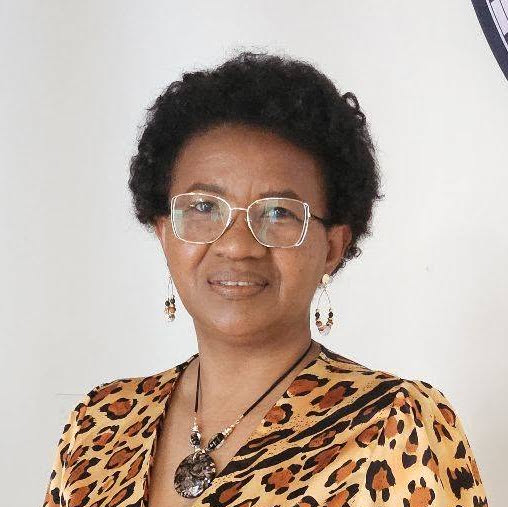
\includegraphics[width=3cm]{../../images/avatar-mum.jpg}};
    \end{tikzpicture}
  \end{minipage}%
  \hfill
  \begin{minipage}[c]{0.80\textwidth}
    \textbf{\fontsize{20 pt}{20 pt}\selectfont Sikazinony DELPHINE}%

    \vspace{0.3 cm}

    \normalsize
    \mbox{{\color{black}\footnotesize\faMapMarker*}\hspace*{0.13cm}17330 Courant}%
    \kern 0.25 cm%
    \AND%
    \kern 0.25 cm%
    \mbox{\hrefWithoutArrow{mailto:delphine.sikazinony@gmail.com}{\color{black}{\footnotesize\faEnvelope[regular]}\hspace*{0.13cm}delphine.sikazinony@gmail.com}}%
    \kern 0.25 cm%
    \AND%
    \kern 0.25 cm%
    \mbox{\hrefWithoutArrow{tel:+33-771-874-078}{\color{black}{\footnotesize\faPhone*}\hspace*{0.13cm}+33 (0)7 71 87 40 78}}%
    \kern 0.25 cm%
    \AND%
    \kern 0.25 cm%
    \mbox{
      \hrefWithoutArrow{https://www.linkedin.com/in/delphine-sikazinony-243728214/}{
        \color{black}{\footnotesize\faLinkedinIn}\hspace*{0.13cm}delphine-sikazinony
      }
    }%
    % Permis B avec petit logo voiture
    \kern 0.25 cm%
    \AND%
    \kern 0.25 cm%
    \mbox{
      \hrefWithoutArrow{https://www.permisb.fr/}{
        \color{black}{\footnotesize\faCar}\hspace*{0.13cm}Permis B
      }
    }%
  \end{minipage}
\end{header}

\vspace{0.2 cm}

% Profil

\section{Profil}

\begin{onecolentry}
  Aide soignante ...
\end{onecolentry}

% Expériences professionnelles

\section{Expériences professionnelles}

  \begin{twocolentry}
    {
      \textit{Bernay-Saint-Martin, France}
      
      \textit{Mars 2025 – Aujourd'hui}
    } {
      \textbf{Aide soignante}

      \textit{EHPAD ADMR Bernay-Saint-Martin}
    }
  \end{twocolentry}

  \vspace{0.10 cm}

  \begin{twocolentry}
    {
      \textit{Bernay-Saint-Martin, France}
      
      \textit{Juin 2023 – Mars 2025}
    } {
      \textbf{Agent de soin}

      \textit{EHPAD ADMR Bernay-Saint-Martin}
    }
  \end{twocolentry}

  \vspace{0.10 cm}

  \begin{twocolentry}
    {
      \textit{Saint-Jean d'Angély, France}
      
      \textit{Juil 2021 – Oct 2022}
    } {
      \textbf{Agent de nettoyage}

      \textit{ADEF}
    }
  \end{twocolentry}

\vspace{0.2 cm}

% Stages

\section{Stages}

  \begin{twocolentry} {
    \textit{Montpellier, France}
    
    \textit{Mars – Août 2023}
  } {
    \textbf{Stage de fin d'études}
    
    \textit{INRAE - UMR G-EAU / UMR Innovation}
  }
  \end{twocolentry}

  \vspace{0.10 cm}

  \begin{onecolentry}
    \begin{highlights}
      \item Modélisation de la gestion de la ressource en eau du bassin versant de
      l'Aude dans un contexte de changement climatique (Projet Talanoa Water)
    \end{highlights}
  \end{onecolentry}

  \vspace{0.1 cm}

  \begin{twocolentry}
    {
      \textit{Rabat, Maroc}

      \textit{Fév - Juil 2022}
    }
    {
      \textbf{Stage de fin d'études}

      \textit{Institut Agronomique et Vétérinaire Hassan II - Département
      Génie Rural}
    }
  \end{twocolentry}

  \vspace{0.10 cm}

  \begin{onecolentry}
    \begin{highlights}
      \item Détermination de la consommation et de la productivité de l'eau
      dans le bassin hydraulique de l'Oum Er Rbia
    \end{highlights}
  \end{onecolentry}

  \vspace{0.1 cm}

  \begin{twocolentry}
    {
      \textit{Rabat, Maroc}

      \textit{Juil - Sept 2021}
    }
    {
      \textbf{Stage d'insertion en milieu professionnel}

      \textit{Compagnie d'Aménagement et de Développement Industriel (ADI)}
    }
  \end{twocolentry}

  \vspace{0.10 cm}

  \begin{onecolentry}
    \begin{highlights}
      \item Dimensionnement du réseau projeté pour la reconversion en irrigation
      localisée du secteur RD1 du périmètre de la Tessaout aval
    \end{highlights}
  \end{onecolentry}

\vspace{0.2 cm}
  
% Diplômes et certificats

\section{Diplômes et certificats}

  \begin{twocolentry}
    {
      \textit{Montpellier, France}

      \textit{Sept 2022 – Sept 2023}
    }
    {
      \textbf{Master 2 Science de l'Eau - Eau et Agriculture}

      \textit{Université de Montpellier - Institut Agro Montpellier - AgroParisTech}
    }
  \end{twocolentry}

  \vspace{0.1 cm}

  \begin{twocolentry}
    {
      \textit{Rabat, Maroc}

      \textit{Sept 2019 – Juil 2022}
    }
    {
      \textbf{Ingénieur Génie Rural - Eau, Environnement et Infrastructures}

      \textit{Institut Agronomique et Vétérinaire Hassan II}
    }
  \end{twocolentry}

  \vspace{0.1 cm}

  \begin{twocolentry}
    {
      \textit{Antsiranana, Madagascar}

      \textit{Sept 2015 – Juil 2019}
    }
    {
      \textbf{Baccalauréat générale - Série A2}

      \textit{Ecole Supérieure Polytechnique Antananarivo}
    }
  \end{twocolentry}

\vspace{0.2 cm}

% Compétences

\section{Compétences}
  \begin{onecolentry}
    \textbf{Bureautique:} Microsoft Office
  \end{onecolentry}

  \vspace{0.1 cm}

  \begin{onecolentry}
    \textbf{OS:} Windows, Linux
  \end{onecolentry}

  \vspace{0.1 cm}

  \begin{onecolentry}
    \textbf{Programmation:} R, Python (base), Fortran (base)
  \end{onecolentry}

  \vspace{0.1 cm}

  \begin{onecolentry}
    \textbf{Versioning:} Git, Gitlab, Github
  \end{onecolentry}

  \vspace{0.1 cm}

  \begin{onecolentry}
    \textbf{CI/CD:} Gitlab CI, Github Actions
  \end{onecolentry}

  \vspace{0.1 cm}

  \begin{onecolentry}
    \textbf{Autres:} CAO/DAO (AutoCAD), Epanet, etc.
  \end{onecolentry}

% Fin

\end{document}
